\documentclass{../../STYLEKIT/sahand_q1}
\usepackage{../../STYLEKIT/sahand_q1}

% --- Identity block (required by ContentLaw) ---
\newcommand{\DocID}{DOC00\_TEMPLATE}
\newcommand{\DocVersion}{v0\_1\_2}
\newcommand{\DocStatus}{S0}
\newcommand{\BuildID}{BUILD\_CI}

\title{\textbf{Sahand Account — Q1 PDF Template}\\\large \DocID\ (\DocVersion) — \DocStatus}
\author{Sahand Account Canon}
\date{\today}

\begin{document}
\maketitle

\begin{center}
\begin{tabular}{ll}
\toprule
Contract & QUALITY\_CONTRACT\_v1.2 \\
DocID & \DocID \\
Version & \DocVersion \\
Status & \DocStatus \\
BuildID & \BuildID \\
\bottomrule
\end{tabular}
\end{center}

\tableofcontents

\section{Purpose}
This document is a minimal compile test that exercises:
(1) Latin text, (2) math glyphs, (3) Persian glyphs, (4) a table, (5) a chart, and
(6) the mandatory \texttt{Tests \& Gates} section.

\section{Glyph sanity}
Latin: The quick brown fox jumps over the lazy dog.

Math: $ \int_0^1 x^2\,dx = \frac{1}{3} \quad,\quad \forall \epsilon>0,\ \exists \delta>0.$

Persian: \textfa{این یک تست فونت فارسی است تا مربع های سیاه یا خالی تولید نشوند.}

\section{A table (required)}
\begin{table}[H]
\centering
\caption{Minimal table style test}
\begin{tabularx}{0.9\linewidth}{lY}
\toprule
Key & Value \\
\midrule
A & Uses booktabs + tabularx. \\
B & Should not overflow. \\
C & Persian+Math should render without tofu. \\
\bottomrule
\end{tabularx}
\end{table}

\section{A chart (required)}
\begin{figure}[H]
\centering
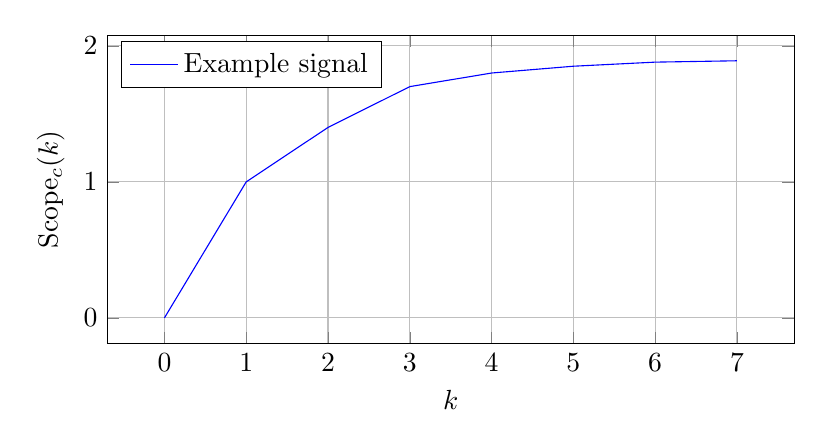
\begin{tikzpicture}
\begin{axis}[
  width=0.85\linewidth,
  height=55mm,
  xlabel={$k$},
  ylabel={Scope$_c(k)$},
  grid=both,
  legend style={at={(0.02,0.98)},anchor=north west},
]
\addplot+[mark=none] coordinates {(0,0) (1,1) (2,1.4) (3,1.7) (4,1.8) (5,1.85) (6,1.88) (7,1.89)};
\addlegendentry{Example signal}
\end{axis}
\end{tikzpicture}
\caption{Inline pgfplots chart (no external assets).}
\end{figure}

\section{A figure (required)}
\begin{figure}[H]
\centering
\fbox{\rule{0pt}{35mm}\rule{0.8\linewidth}{0pt}}
\caption{Figure placeholder (replace with vector PDF/SVG later).}
\end{figure}

\TestsAndGatesSection
\begin{itemize}
\item Gate G2 (Missing character): PASS iff log contains zero ``Missing character:'' lines.
\item Gate G3 (Overfull hbox): PASS iff overfull count $\le 5$ (template should be 0).
\item Gate G7 (Registry/Annex): PASS iff SHA256SUMS + ANNEX + SQLite record exist (later stage).
\end{itemize}

\end{document}
